\documentclass[border=15pt,tikz]{standalone}
\usepackage{amsmath}
\usetikzlibrary{arrows.meta, fit, positioning, backgrounds, matrix}
\usepackage[outline]{contour}
\contourlength{1.4pt}

\usepackage{helvet}
\renewcommand{\familydefault}{\sfdefault}
\usepackage{sansmath}
\sansmath

% --- COLOR DEFINITIONS ---
\usepackage{xcolor}
\colorlet{myred}{red!80!black}
\colorlet{myblue}{blue!80!black}
\colorlet{mygreen}{green!60!black}
\colorlet{myorange}{orange!70!red!60!black}
\colorlet{myviolet}{violet!70!black}
\colorlet{mydarkred}{red!30!black}
\colorlet{mydarkblue}{blue!40!black}
\colorlet{mydarkgreen}{green!30!black}
\colorlet{mydarkviolet}{violet!40!black}

% --- STYLES ---
\tikzset{
  >=latex,
  base node/.style={thick, circle, minimum size=22pt, inner sep=1pt, align=center, font=\scriptsize},
  node graph/.style={base node, draw=mygreen!40!black, fill=mygreen!15},
  op block/.style={thick, rounded corners=4pt, draw=myblue!40!black, fill=myblue!12, minimum width=4.6cm, minimum height=0.62cm, align=center, font=\scriptsize, inner sep=3pt},
  op block small/.style={op block, minimum width=2.15cm},
  cell/.style={draw=mydarkviolet, thick, minimum width=0.85cm, minimum height=0.62cm, align=center, font=\scriptsize, fill=myviolet!6},
  cell win/.style={cell, fill=myviolet!30, draw=myviolet, ultra thick},
  inter edge/.style={thick, mygreen, shorten >=2pt, shorten <=2pt},
  intra edge/.style={thick, dashed, mydarkgreen!70!black, shorten >=2pt, shorten <=2pt},
  flow arrow/.style={->, thick, line width=1.5pt, draw=black!60},
  bad arrow/.style={->, thick, myred, dashed},
  good arrow/.style={->, thick, mygreen!50!black},
  label/.style={font=\small\bfseries, align=center},
  desc/.style={font=\scriptsize, align=center, text=black!80},
  box/.style={draw, thick, rounded corners=6pt, inner sep=14pt, fill opacity=0.05}
}

\begin{document}

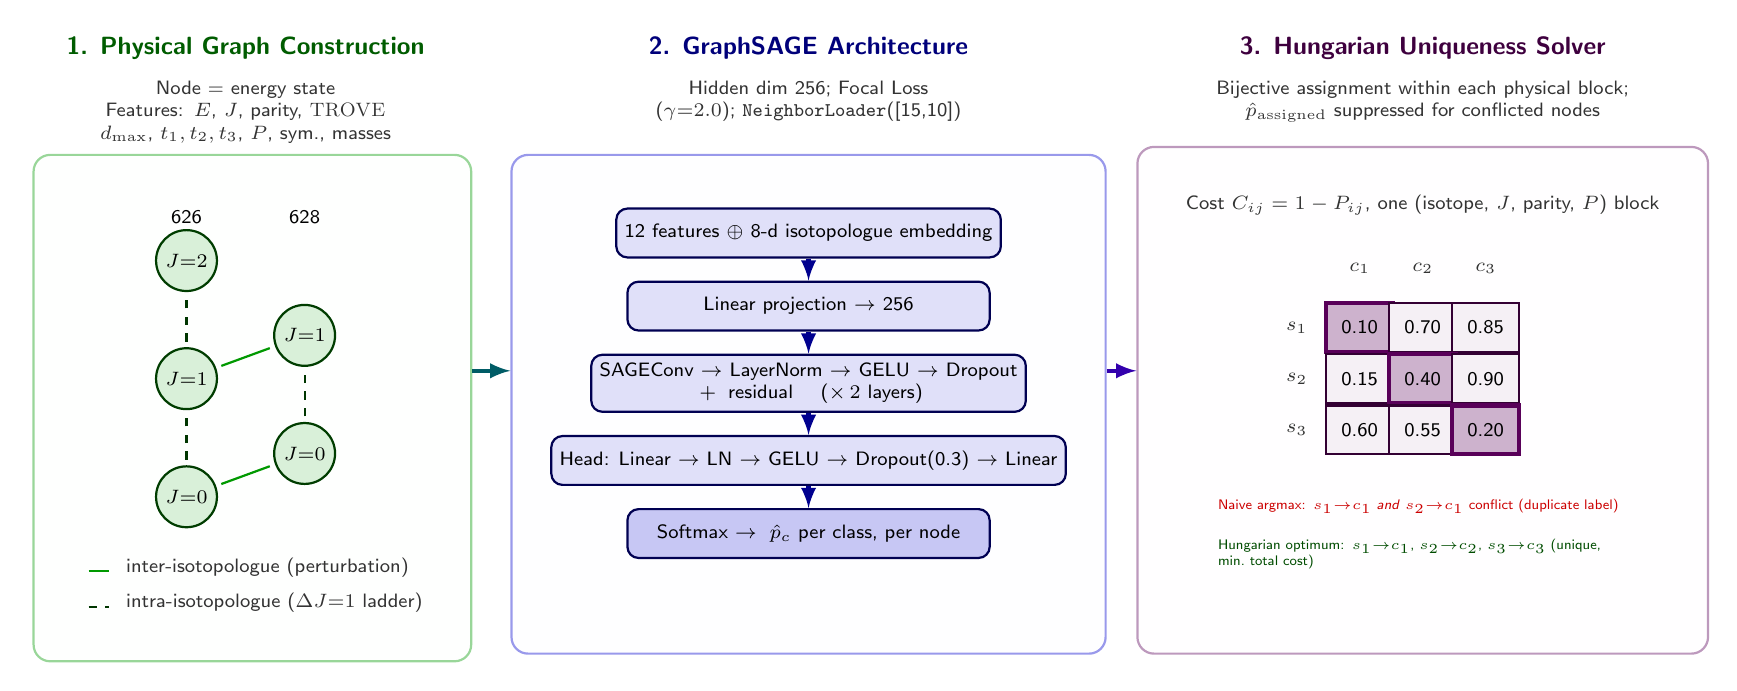
\begin{tikzpicture}[font=\sffamily]

  % =================================================================================
  % PANEL 1: PHYSICAL GRAPH CONSTRUCTION
  % =================================================================================

  \node[label, font=\scriptsize] (col626) at (0.0, 2.85) {626};
  \node[label, font=\scriptsize] (col628) at (1.5, 2.85) {628};

  \node[node graph] (A0) at (0.0, -0.7) {$J{=}0$};
  \node[node graph] (A1) at (0.0, 0.8) {$J{=}1$};
  \node[node graph] (A2) at (0.0, 2.3) {$J{=}2$};
  \node[node graph] (B0) at (1.5, -0.15) {$J{=}0$};
  \node[node graph] (B1) at (1.5, 1.35) {$J{=}1$};

  % Intra-isotopologue rotational ladder (Delta J = 1)
  \draw[intra edge] (A0) -- (A1);
  \draw[intra edge] (A1) -- (A2);
  \draw[intra edge] (B0) -- (B1);

  % Inter-isotopologue perturbation edges (shared polyad, J, parity)
  \draw[inter edge] (A0) -- (B0);
  \draw[inter edge] (A1) -- (B1);

  \node[label, mygreen!60!black] at (0.75, 5.0) (Title1) {1. Physical Graph Construction};
  \node[desc, below=1pt of Title1, text width=5.3cm] {Node = energy state\\Features: $E$, $J$, parity, \textsc{TROVE} $d_{\max}$, $t_1,t_2,t_3$, $P$, sym., masses};

  % Legend: explicit coordinates, one line per entry (no text width, no wrapping)
  \node[desc, anchor=west] (leg1a) at (-1.45, -1.6) {\tikz{\draw[inter edge] (0,0) -- (0.4,0);}\, inter-isotopologue (perturbation)};
  \node[desc, anchor=west] (leg1b) at (-1.45, -2.05) {\tikz{\draw[intra edge] (0,0) -- (0.4,0);}\, intra-isotopologue ($\Delta J{=}1$ ladder)};

  % Invisible corners give all three panels identical top/bottom edges
  \coordinate (p1t) at (0.75, 3.15);
  \coordinate (p1b) at (0.75, -2.2);
  \begin{pgfonlayer}{background}
    \node[box, fit=(col626) (col628) (A0) (A2) (B0) (B1) (leg1a) (leg1b) (p1t) (p1b), fill=mygreen!5, draw=mygreen!40] (panel1) {};
  \end{pgfonlayer}


  % =================================================================================
  % PANEL 2: GRAPHSAGE ARCHITECTURE
  % =================================================================================

  \node[op block] (G1) at (7.9, 2.65) {12 features $\oplus$ 8-d isotopologue embedding};
  \node[op block] (G2) [below=0.28cm of G1] {Linear projection $\rightarrow$ 256};
  \node[op block] (G3) [below=0.28cm of G2] {SAGEConv $\rightarrow$ LayerNorm $\rightarrow$ GELU $\rightarrow$ Dropout \\ ${}+{}$ residual \quad ($\times\,2$ layers)};
  \node[op block] (G4) [below=0.28cm of G3] {Head: Linear $\rightarrow$ LN $\rightarrow$ GELU $\rightarrow$ Dropout(0.3) $\rightarrow$ Linear};
  \node[op block, fill=myblue!22] (G5) [below=0.28cm of G4] {Softmax $\rightarrow\; \hat p_c$ per class, per node};

  \draw[flow arrow, draw=myblue!70!black] (G1) -- (G2);
  \draw[flow arrow, draw=myblue!70!black] (G2) -- (G3);
  \draw[flow arrow, draw=myblue!70!black] (G3) -- (G4);
  \draw[flow arrow, draw=myblue!70!black] (G4) -- (G5);

  \coordinate (p2t) at (7.9, 3.15);
  \coordinate (p2b) at (7.9, -2.2);
  \begin{pgfonlayer}{background}
    \node[box, fit=(G1) (G2) (G3) (G4) (G5) (p2t) (p2b), fill=myblue!5, draw=myblue!40] (panel2) {};
  \end{pgfonlayer}

  \node[label, myblue!60!black] at (7.9, 5.0) (Title2) {2. GraphSAGE Architecture};
  \node[desc, below=1pt of Title2, text width=4.8cm] {Hidden dim 256; Focal Loss ($\gamma{=}2.0$); \texttt{NeighborLoader}([15,10])};


  % =================================================================================
  % PANEL 3: HUNGARIAN UNIQUENESS SOLVER
  % =================================================================================

  \node[label, myviolet!70!black] at (15.7, 5.0) (Title3) {3. Hungarian Uniqueness Solver};
  \node[desc, below=1pt of Title3, text width=5.6cm] {Bijective assignment within each physical block; $\hat p_{\mathrm{assigned}}$ suppressed for conflicted nodes};

  \node[desc] (solverIntro) at (15.7, 3.0) {Cost $C_{ij}=1-P_{ij}$, one (isotope, $J$, parity, $P$) block};

  % Column / row headers
  \node[desc] (c1h) at (14.9, 2.2) {$c_1$};
  \node[desc] (c2h) at (15.7, 2.2) {$c_2$};
  \node[desc] (c3h) at (16.5, 2.2) {$c_3$};
  \node[desc] (s1h) at (14.1, 1.45) {$s_1$};
  \node[desc] (s2h) at (14.1, 0.8)  {$s_2$};
  \node[desc] (s3h) at (14.1, 0.15) {$s_3$};

  \node[cell win] (s1c1) at (14.9, 1.45) {0.10};
  \node[cell]     (s1c2) at (15.7, 1.45) {0.70};
  \node[cell]     (s1c3) at (16.5, 1.45) {0.85};
  \node[cell]     (s2c1) at (14.9, 0.8)  {0.15};
  \node[cell win] (s2c2) at (15.7, 0.8)  {0.40};
  \node[cell]     (s2c3) at (16.5, 0.8)  {0.90};
  \node[cell]     (s3c1) at (14.9, 0.15) {0.60};
  \node[cell]     (s3c2) at (15.7, 0.15) {0.55};
  \node[cell win]  (s3c3) at (16.5, 0.15) {0.20};

  \node[desc, font=\tiny, myred, below=16pt of s3h, xshift=1.6cm, text width=5.2cm, align=left]
    (naive) {Naive argmax: $s_1{\to}c_1$ \emph{and} $s_2{\to}c_1$ conflict (duplicate label)};
  \node[desc, font=\tiny, mygreen!50!black, below=2pt of naive, text width=5.2cm, align=left]
    (opt) {Hungarian optimum: $s_1{\to}c_1$, $s_2{\to}c_2$, $s_3{\to}c_3$ (unique, min.\ total cost)};

  \coordinate (p3t) at (15.7, 3.15);
  \coordinate (p3b) at (15.7, -2.2);
  \begin{pgfonlayer}{background}
    \node[box, fit=(solverIntro) (c1h) (s1h) (s1c1) (s3c3) (naive) (opt) (p3t) (p3b), fill=myviolet!5, draw=myviolet!40] (panel3) {};
  \end{pgfonlayer}


  % =================================================================================
  % MACRO FLOW CONNECTIONS
  % =================================================================================

  % Horizontal arrows at a fixed height so panel-size differences don't slant them
  \draw[flow arrow, draw=mygreen!60!blue]   (panel1.east |- 0,0.9) -- (panel2.west |- 0,0.9);
  \draw[flow arrow, draw=myblue!60!violet]  (panel2.east |- 0,0.9) -- (panel3.west |- 0,0.9);

\end{tikzpicture}

\end{document}
